\section{Évaluation de l'hypothèse d'efficience}
\label{section:4.2-HYPOTHESE-EFFICIENCE}

	%%%
	%%% Introduction / Transition.
	%%%
	Suite à la validation de l'hypothèse d'efficacité (convergence de la méthode, cf. \textsc{Section~\ref{section:4.1-HYPOTHESE-EFFICACITE}}), nous voulons déterminer les paramètres optimaux de la méthode afin de converger le plus rapidement vers la vérité terrain.
	Nous aimerions donc vérifier l'hypothèse suivante :

	%%%
	%%% Formulation des hypothèses.
	%%%
	\begin{tcolorbox}[
		title=\faVial~\textbf{Hypothèse d'efficience}~\faVial,
		colback=colorTcolorboxHypothesis!15,
		colframe=colorTcolorboxHypothesis!75,
		width=\linewidth
	]

		% Hypothèse.
		\textguillemets{\textbf{
			La vitesse de convergence du \textit{clustering} interactif peut être optimisée en ajustant différents paramètres afin de minimiser la charge de travail de l'opérateur.
			Nous étudions en particulier l'influence sur le nombre de contraintes requis du prétraitement des données, de la vectorisation des données, de l'échantillonnage des contraintes à annoter et du \textit{clustering} sous contraintes.
		}} \\
		
		% Figure.
		La \textsc{Figure~\ref{figure:4.2-HYPOTHESE-EFFICIENCE}} illustre cette hypothèse et l'espoir d'une convergence "optimale" d'une base d'apprentissage en cours de construction vers sa vérité terrain.
		%
		\begin{figure}[H]  % keep [H] to be in the tcolorbox.
			\centering
			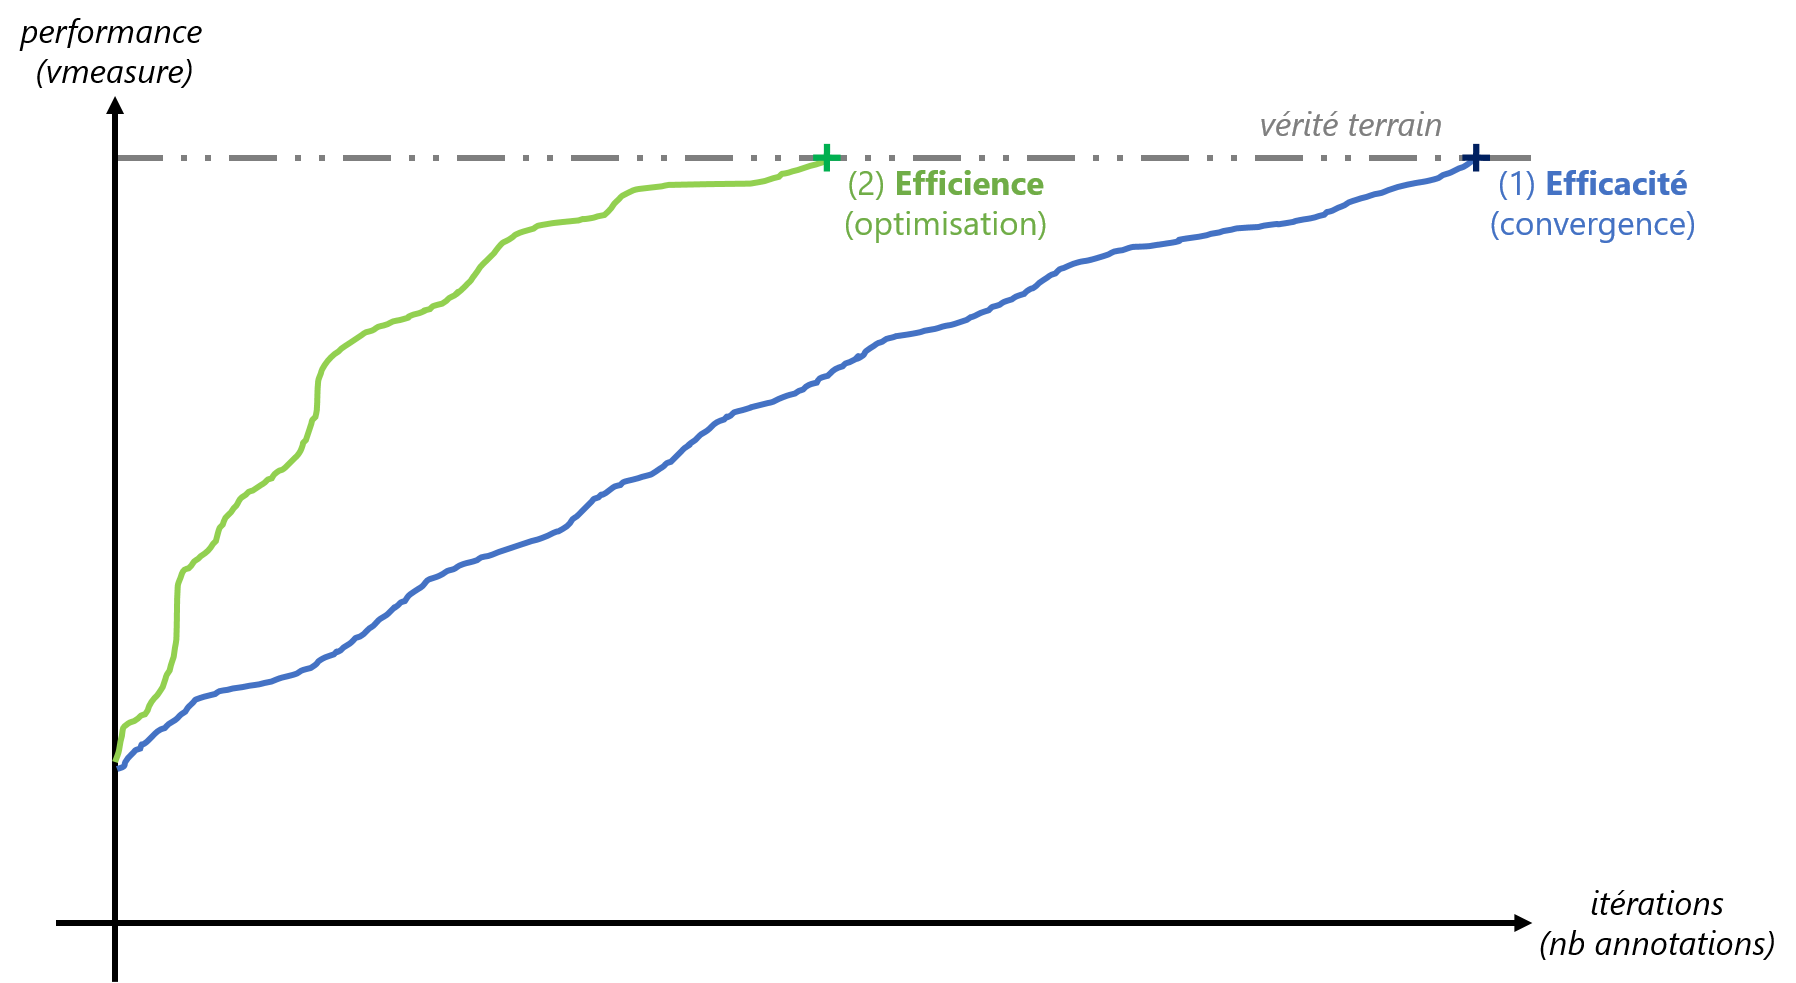
\includegraphics[width=0.95\textwidth]{figures/hypotheses-02-efficience}
			\caption{
				Illustration des études réalisées sur le \textit{clustering} interactif (\textit{étape 2/6}) en schématisant l'évolution de la performance (\textit{accord avec la vérité terrain calculé en v-measure}) d'une base d'apprentissage en cours de construction en fonction du nombre d'itérations de la méthode (\textit{nombre d'annotations par un expert métier}).
			}
			\label{figure:4.2-HYPOTHESE-EFFICIENCE}
		\end{figure}
	\end{tcolorbox}
	
	% Résumé de l'étude.
	Afin de vérifier cette hypothèse, nous mettons en place une expérience de ré-annotation d'une base d'apprentissage (qui servira ici de vérité terrain) à l'aide de notre méthode, en simulant l'annotation d'un expert, et nous réalisons l'analyse statistique de la taille d'effets de différents paramètres sur la \textbf{vitesse de convergence} du \textit{clustering} itératif (cf. \textsc{Section~\ref{section:4.2.1-ETUDE-OPTIMISATION}}).
	
		
	%%%
	%%% Subsection 4.2.1: Étude d'optimisation des paramètres d'implémentation en analysant leurs tailles d'effets sur la vitesse de création d'une base d'apprentissage.
	%%%
	\subsection{Étude d'optimisation des paramètres d'implémentation en analysant leurs tailles d'effets sur la vitesse de création d'une base d'apprentissage}
	\label{section:4.2.1-ETUDE-OPTIMISATION}

		% Objectif de l'expérience.
		Nous voulons étudier l'influence des paramètres de notre implémentation du \textit{clustering} interactif sur la vitesse de création d'une base d'apprentissage pour un assistant conversationnel.
		Nous allons donc compléter le protocole expérimental de l'étude de convergence en \textsc{Section~\ref{section:4.1.1-ETUDE-CONVERGENCE}} visant à simuler la création d'une base d'apprentissage.
			
		% Référence articles.
		\begin{leftBarInformation}
			Cette étude a été l'objet d'une présentation à la conférence \texttt{EGC (Extraction et Gestion des Connaissances)}~(\cite{schild-etal:2021:conception-iterative-semisupervisee}), et d'une extension dans le journal \texttt{IJDWM (International Journal of Data Warehousing and Mining)}~(\cite{schild-etal:2022:iterative-semisupervised-design}).
			\footnote{
				Les résultats et la discussion de ces articles ont été mis à jour et réécrits pour mieux s'intégrer au discours ce manuscrit.
			}
		\end{leftBarInformation}

		%%% Protocole expérimental.
		\subsubsection{Protocole expérimental}
			
			% Axiome.
			\begin{leftBarWarning}
				Comme dans l'étude précédente, nous supposons que l'expert métier connaît parfaitement le domaine traité dans ce jeu de données, et qu'il est capable de caractériser sans ambiguïté la similitude entre deux données issues de cet ensemble.
				Cependant, cette hypothèse forte n'est pas toujours vérifiée en pratique, surtout lorsque l'on manipule des données non structurées.
				L'impact de ce point sur les résultats obtenus est discuté en fin de partie, et nous nous y intéressons plus en détails dans la \textsc{Section~\ref{section:4.6-HYPOTHESE-ROBUSTESSE}} (hypothèse de robustesse).
			\end{leftBarWarning}
			
			% Pseudo-code.
			Pour résumer le protocole expérimental adapté, vous pouvez vous référer au pseudo-code décrit dans \textsc{Algorithme~\ref{algorithm:4.2.1-ETUDE-OPTIMISATION-PROTOCOLE}}.
			
			\begin{algorithm}
				\KwData{jeu de données annotées (vérité terrain)}
				\KwIn{combinaisons d'algorithmes et de paramètres à tester}
				%
				\ForEach{combinaison d'algorithmes et de paramètres à tester}{
					\textbf{initialisation (données)}: récupérer les données et la vérité terrain \;
					\textbf{initialisation (contraintes)}: créer une liste vide de contraintes \;
					\textbf{prétraitement}: supprimer le bruit dans les données \;
					\textbf{vectorisation}: transformer les données en vecteurs \;
					\textbf{clustering initial}: regrouper les données par similarité des vecteurs \;
					\textbf{évaluation}: estimer l'équivalence entre le \textit{clustering} et la vérité terrain \;
					\Repeat{annotation de toutes les contraintes possibles}{
						\textbf{échantillonnage}: sélectionner de nouvelles contraintes à annoter \;
						\textbf{simulation d'annotation}: déterminer les contraintes avec la vérité terrain \;
						\textbf{intégration}: ajouter les nouvelles contraintes au gestionnaire de contraintes \;
						\textbf{clustering}: regrouper les données par similarité avec les contraintes \;
						\textbf{évaluation}: estimer l'équivalence entre le \textit{clustering} et la vérité terrain \;
					}
				}
				\textbf{analyse}: déterminer les tailles d'effets des algorithmes et paramètres \;
				%
				\KwResult{meilleures combinaisons d'algorithmes et de paramètres}
				%
				\caption{\textit{
					Description en pseudo-code du protocole expérimental de l'étude d'optimisation de la convergence du \textit{clustering} interactif vers une vérité terrain pré-établie.
				}}
				\label{algorithm:4.2.1-ETUDE-OPTIMISATION-PROTOCOLE}
			\end{algorithm}
			
			% Détails de l'expérience.
			En s'appuyant sur les résultats précédemment obtenus,
			nous allons analyser l'influence des différentes tâches employées (\textbf{prétraitement}, \textbf{vectorisation}, \textbf{clustering sous contraintes}, \textbf{échantillonnage}) et de leurs paramètres sur la vitesse de convergence vers la vérité terrain.
			% Description implémentation de l'interactive clustering.
			Nous utilisons à nouveau le jeu de données \texttt{Bank Cards (v1.0.0)} (cf. annexe~\ref{annex:A.1-DATASET-BANK-CARDS}) comme vérité terrain, sur lequel nous testons $192$ combinaisons de paramétrages, et chaque tentative est répétée $5$ fois pour contrer les aléas statistiques de certains algorithmes.
			Pour plus de détails sur ces algorithmes, référez-vous à la \textsc{Section~\ref{section:3.3-DESCRIPTION-IMPLEMENTATION}}.
			
			% Description de l'évaluation et Seuils d'évaluation.
			Comme lors de l'étude sur la convergence de la méthode, nous nous intéressons à l'évolution de la \texttt{v-measure} (\cite{rosenberg-hirschberg:2007:vmeasure-conditional-entropybased}) entre la vérité terrain et notre segmentation des données obtenue, et nous affinons notre évaluation en portant attention aux trois seuils d'annotations suivants :
			\begin{enumerate}
				\item le cas d'une \textbf{annotation partielle}, correspondant au nombre d'itérations nécessaires à la méthode pour avoir $90$\% de \texttt{v-measure}, c'est-à-dire un état de semi-parcours vers une convergence totale\footnote{
					Le seuil de $90$\% a été choisi au cours de l'étude de convergence (cf. hypothèse d'efficacité, \textsc{Section~\ref{section:4.1-HYPOTHESE-EFFICACITE}}, coude de la \textsc{Figure~\ref{figure:4.1.1-ETUDE-CONVERGENCE-EVOLUTION}}).
				} ;
				\item le cas d'une \textbf{annotation suffisante}, correspondant au nombre d'itérations nécessaires à la méthode pour avoir $100$\% de \texttt{v-measure}, c'est-à-dire avoir suffisamment de contraintes annotées par l'expert métier pour retrouver la vérité terrain ;
				\item le cas d'une \textbf{annotation exhaustive}, correspondant au nombre d'itérations nécessaires à la méthode pour parcourir toutes les contraintes possibles sur les données, et ainsi retranscrire exhaustivement la vision de l'expert métier\footnote{
					Une annotation est a priori inutilisable en pratique (demande trop de contraintes, cf. hypothèse d'efficacité, \textsc{Section~\ref{section:4.1-HYPOTHESE-EFFICACITE}}), nous l'étudions toutefois pour avoir un point de comparaison.
				}.
			\end{enumerate}
			
			% Description de l'analyse ANOVA.
			Enfin, nous utilisons une \texttt{ANOVA} à mesures répétées (\cite{girden:1992:anova}) afin de déterminer l'effet des paramètres de notre implémentation sur le nombre d'annotations requis pour converger vers la vérité terrain. Le test de \texttt{Tukey (HSD)} (\cite{tukey:1949:comparing-individual-means}) est utilisé pour les comparaisons post-hoc.
			
			% Référence scripts.
			\begin{leftBarInformation}
				Les scripts de l'expérience, réalisés avec des \textit{notebooks} Python (\cite{van-rossum-drake:2009:python-reference-manual}) et des scripts R (\cite{r-core-team:2017:language-environment-statistical}), sont disponibles dans un dossier dédié de~\cite{schild:2021:cognitivefactory-interactiveclusteringcomparativestudy}.
			\end{leftBarInformation}

		%%% Résultats.
		\subsubsection{Résultats obtenus}
		
			%%% Analyse d'une annotation partielle.
			Pour obtenir une \textbf{annotation partielle} (\textit{atteindre une \texttt{v-measure} de $90$\%}), la moyenne des itérations est de $59.04$ (min: $11$, max: $315$, écart-type: $42.14$), soit une moyenne de $2~951.81$ annotations (min: $550$, max: $15~750$, écart-type: $2~106.72$).
			La \textsc{Figure~\ref{figure:4.2.1-ETUDE-OPTIMISATION-HISTOGRAMME-ANNOTATION-PARTIELLE}} représente la répartition de ces itérations au cours des différentes tentatives.
			On peut noter les deux cas intéressants suivants :
			\begin{itemize}
				\item[$\bullet$] Les tentatives les plus rapides furent celles avec un prétraitement des données \texttt{prep.no} ou \texttt{prep.simple} ou \texttt{prep.lemma}, une vectorisation des données \texttt{vect.tfidf}, un \textit{clustering} sous contraintes \texttt{clust.hier.sing}, et un échantillonnage de contraintes \texttt{samp.closest.diff}. Ces tentatives ont requis $11$ itérations, soit $550$ annotations, dont $299$ (respectivement $304$ et $281$) contraintes \texttt{MUST-LINK}.
				\item[$\bullet$] Les tentatives les plus lentes furent celles avec un prétraitement des données \texttt{prep.no}, une vectorisation des données \texttt{vect.tfidf}, un \textit{clustering} sous contraintes \texttt{clust.spec}, et un échantillonnage de contraintes \texttt{samp.farthest.same}. Ces tentatives ont requis $315$ itérations, soit $15~750$ annotations, dont $1~032$ contraintes \texttt{MUST-LINK}.
			\end{itemize}
			%
			\begin{figure}[!htb]
				\centering
				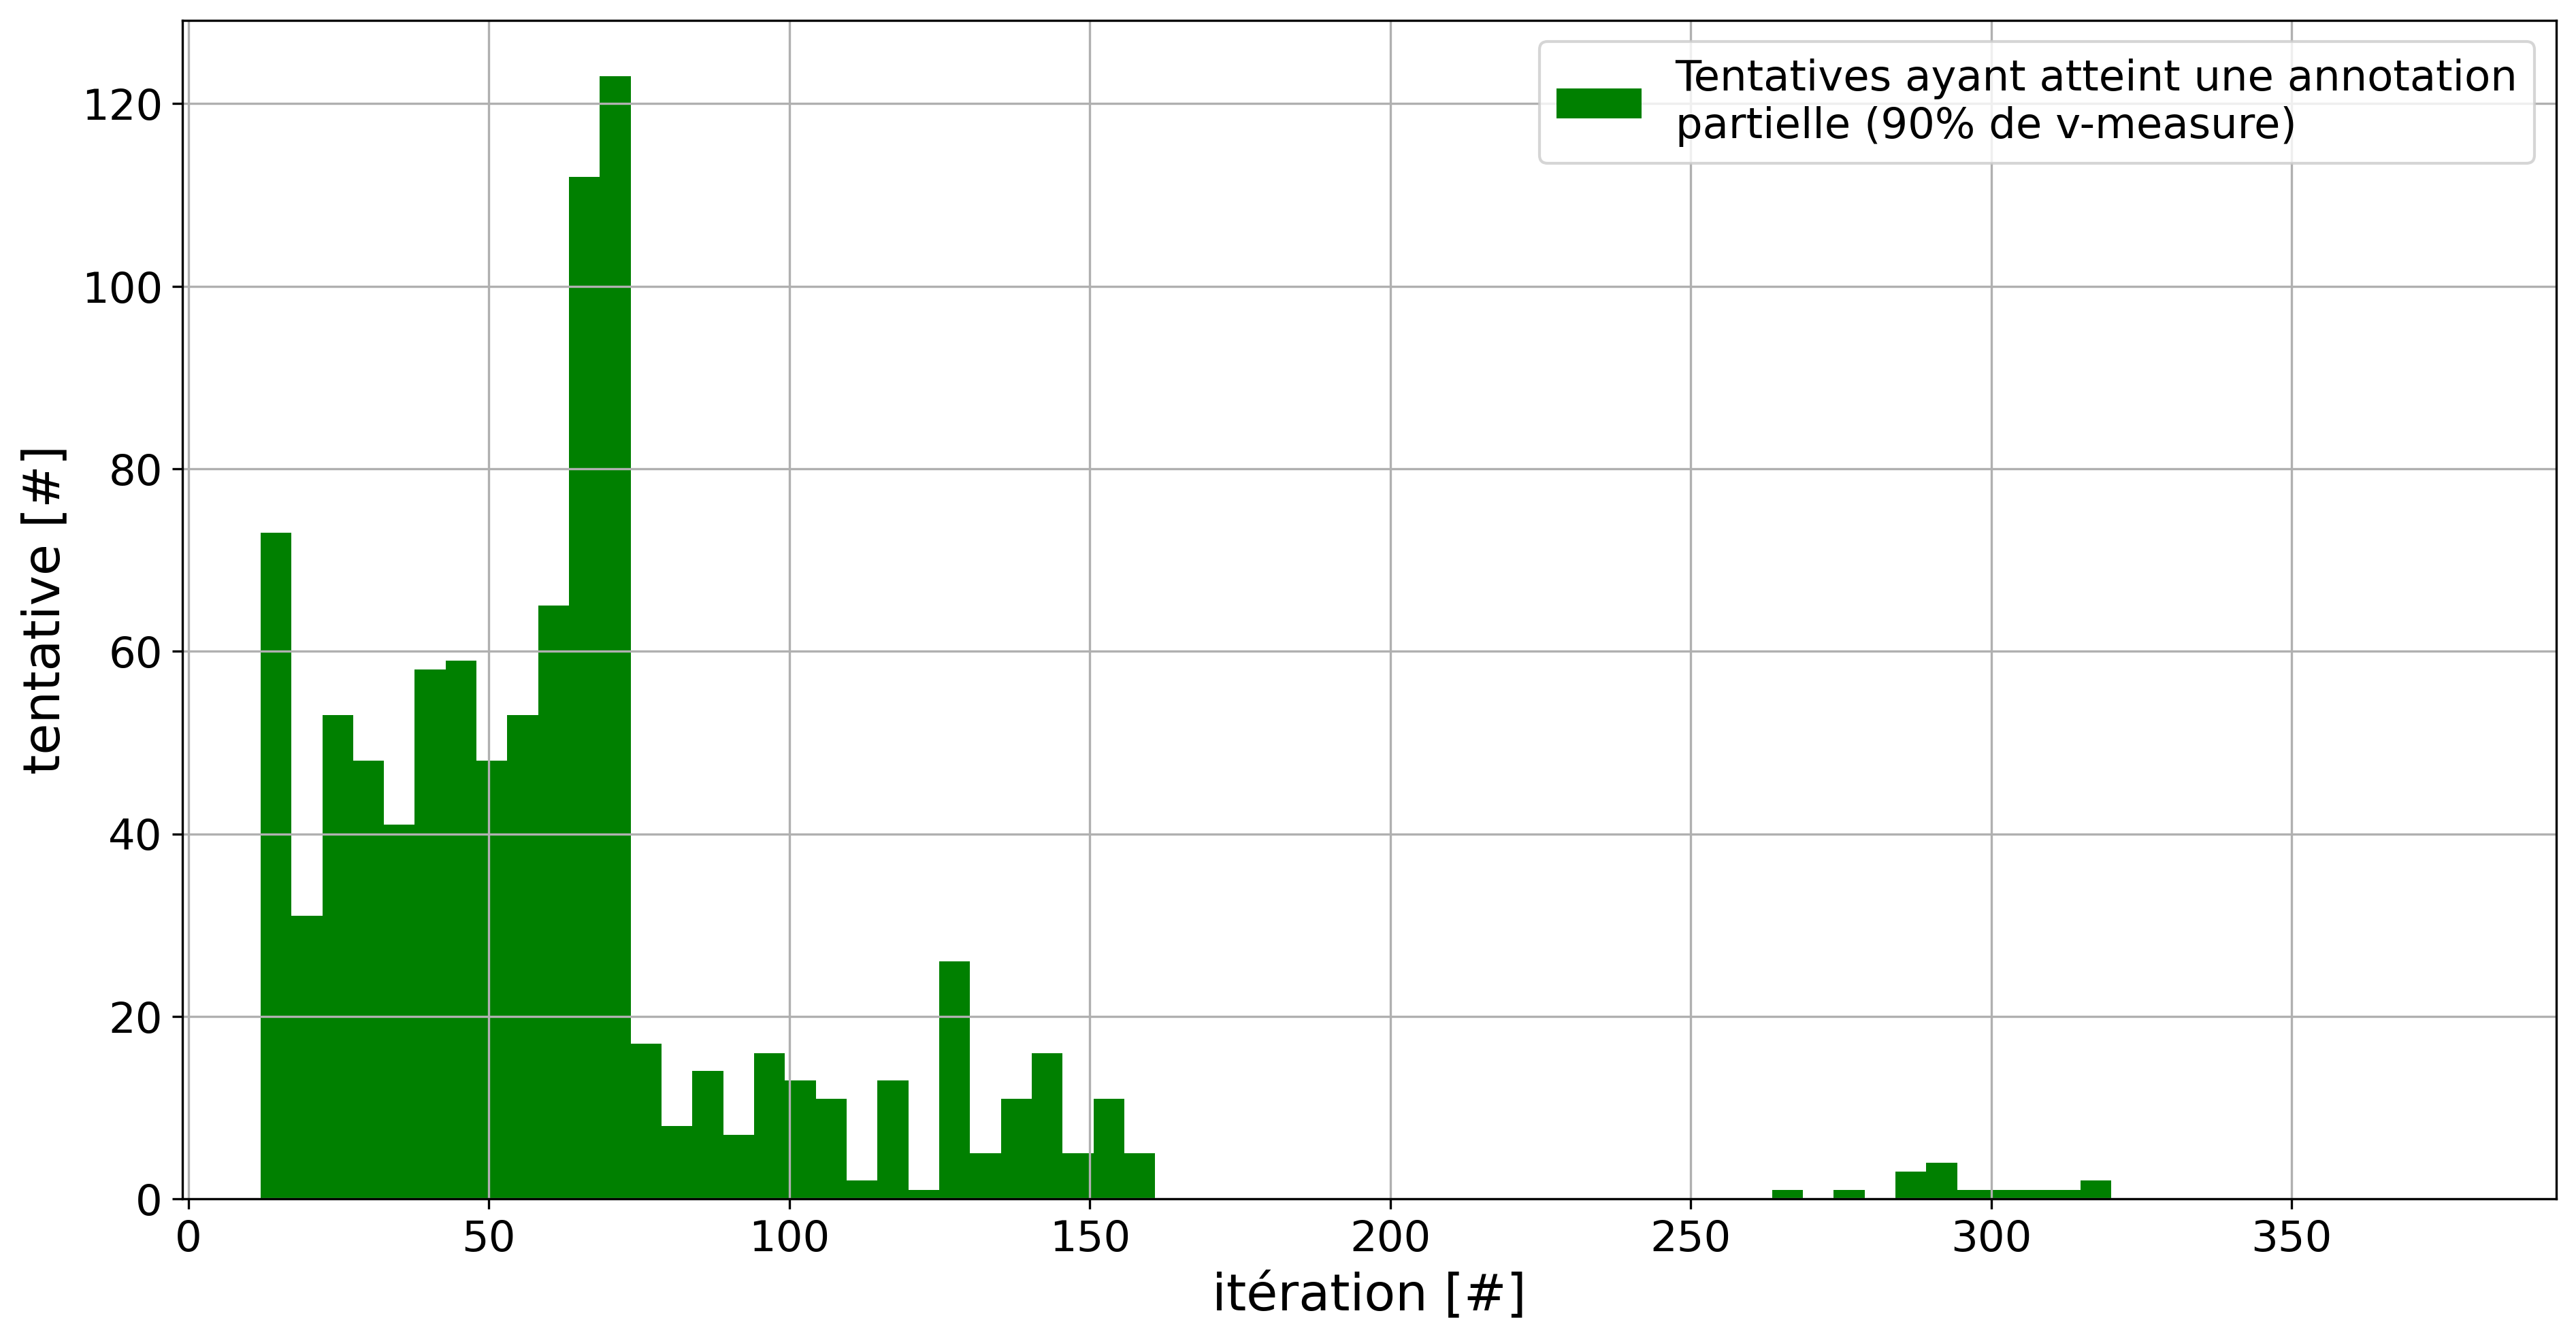
\includegraphics[width=0.90\textwidth]{figures/etude-efficience-histogramme-annotation-partielle}
				\caption{
					Répartition des tentatives en fonction de l'itération de la méthode à laquelle elles atteignent le seuil d'une annotation partielle, c'est-à-dire l'itération à laquelle elles parviennent à $90$\% de \texttt{v-measure} entre un résultat obtenu et la vérité terrain.
					L'histogramme est réduit à $60$ pics pour simplifier l'affichage.
				}
				\label{figure:4.2.1-ETUDE-OPTIMISATION-HISTOGRAMME-ANNOTATION-PARTIELLE}
			\end{figure}
			%
			La \textsc{Table~\ref{table:4.2.1-ETUDE-OPTIMISATION-ANOVA-ANNOTATION-PARTIELLE}} retranscrit l'influence de chacun des paramètres sur le nombre d'itérations nécessaires pour atteindre une \textbf{annotation partielle} (\textit{atteindre une \texttt{v-measure} de $90$\%}).
			Les analyses de variance mettent en relief l'effet significatif sur cette convergence du prétraitement (\texttt{eta-carré}: $0.320$, \texttt{p-valeur}: $< 10^{-3}$), de la vectorisation (\texttt{eta-carré}: $0.388$, \texttt{p-valeur}: $< 10^{-3}$), du \textit{clustering} (\texttt{eta-carré}: $0.866$, \texttt{p-valeur}: $< 10^{-3}$) et de l'échantillonnage (\texttt{eta-carré}: $0.968$, \texttt{p-valeur}: $< 10^{-3}$).
			L'analyse post-hoc de ces effets indique que le meilleur paramétrage moyen pour atteindre une \textbf{annotation partielle} repose sur le prétraitement \texttt{prep.simple}, le vectorisation \texttt{vect.tfidf}, le \textit{clustering} \texttt{clust.hier.avg}, et l'échantillonnage \texttt{samp.closest.diff}. La moyenne du nombre d'itération requis pour ce paramétrage est de $19.00$ (écart-type: $0.79$), soit $950$ annotations (écart-type: $39.34$).
			%
			\begin{table}[!htb]
				\begin{center}
				\begin{tabular}{|c|c|c|c|c|c|c|}
					\hline
					% ENTETE DU TABLEAU
					\rowcolor{colorTableHeader!15}
					\multicolumn{2}{|c|}{ \shortstack{Description des \\ facteurs analysés } }
						& \multicolumn{3}{c|}{ \shortstack{ Description statistique \\ des itérations } }
						& \multicolumn{2}{c|}{ \shortstack{ Description des \\ tailles d'effets } }
						\tabularnewline
						\hline
					\rowcolor{colorTableHeader!15}
					Facteur
						& Niveau 
						& Moyenne
						& Rang
						& SE
						& \texttt{ $ \eta^{2} $ }
						& \texttt{p-valeur}
						\tabularnewline
						\hline
					
					% PRETRAITEMENT
					\multirow{4}{*}{prétraitement}
						& \texttt{prep.simple}
						& $61.90$
						& (1)
						& \multirow{4}{*}{ $0.32$ }
						& \multirow{4}{*}{ $0.320$ }
						& \multirow{4}{*}{ \shortstack{ $< 10^{-3}$ \\ ($***$) } }
						\tabularnewline
						\cline{2-4}
						
						& \texttt{prep.lemma}
						& $63.08$
						& (2)
						&
						&
						&
						\tabularnewline
						\cline{2-4}
						
						& \texttt{prep.no}
						& $63.70$
						& (2)
						&
						& 
						&
						\tabularnewline
						\cline{2-4}
						
						& \texttt{prep.filter}
						& $71.90$
						& (4)
						&
						&
						&
						\tabularnewline
						\hline
					
					% VECTORISATION
					\multirow{2}{*}{vectorisation}
						& \texttt{vect.tfidf}
						& $60.61$
						& (1)
						& \multirow{2}{*}{ $0.29$ }
						& \multirow{2}{*}{ $0.388$ }
						& \multirow{2}{*}{ \shortstack{$< 10^{-3}$ \\ ($***$) } }
						\tabularnewline
						\cline{2-4}
						
						& \texttt{vect.frcorenewsmd}
						& $63.08$
						& (2)
						&
						&
						&
						\tabularnewline
						\hline
					
					% CLUSTERING
					\multirow{6}{*}{clustering}
						& \texttt{clust.hier.avg}
						& $50.64$
						& (1)
						& \multirow{6}{*}{ $0.35$ }
						& \multirow{6}{*}{ $0.866$ }
						& \multirow{6}{*}{ \shortstack{ $< 10^{-3}$ \\ ($***$) } }
						\tabularnewline
						\cline{2-4}
						
						& \texttt{clust.kmeans.cop}
						& $52.43$
						& (2)
						&
						&
						&
						\tabularnewline
						\cline{2-4}
						
						& \texttt{clust.hier.sing}
						& $54.08$
						& (3)
						&
						& 
						&
						\tabularnewline
						\cline{2-4}
						
						& \texttt{clust.hier.ward}
						& $72.41$
						& (4)
						&
						& 
						&
						\tabularnewline
						\cline{2-4}
						
						& \texttt{clust.hier.comp}
						& $73.48$
						& (5)
						&
						&
						&
						\tabularnewline
						\cline{2-4}
						
						& \texttt{clust.spec}
						& $87.84$
						& (6)
						&
						& 
						&
						\tabularnewline
						\hline
					
					% ECHANTILLONNAGE
					\multirow{4}{*}{échantillonnage}
						& \texttt{samp.closest.diff}
						& $33.66$
						& (1)
						& \multirow{4}{*}{ $0.32$ }
						& \multirow{4}{*}{ $0.968$ }
						& \multirow{4}{*}{ \shortstack{ $< 10^{-3}$ \\ ($***$) } }
						\tabularnewline
						\cline{2-4}
						
						& \texttt{samp.random.same}
						& $48.24$
						& (2)
						&
						&
						&
						\tabularnewline
						\cline{2-4}
						
						& \texttt{samp.random.full}
						& $65.83$
						& (3)
						&
						& 
						&
						\tabularnewline
						\cline{2-4}
						
						& \texttt{samp.farhtest.same}
						& $112.86$
						& (4)
						&
						&
						&
						\tabularnewline
						\hline
				\end{tabular}
				\end{center}
				\caption{
					ANOVA du nombre d'itérations nécessaires pour l'obtention de $90$\% de v-mesure. Les ($\textit{*}$) dénotent le niveau de significativité ($\alpha=0.05$). Pour les effets significatifs, les chiffres précisés entre parenthèses dans la colonne \texttt{Moyenne} indiquent le classement des niveaux selon les analyses post-hoc.
				}
				\label{table:4.2.1-ETUDE-OPTIMISATION-ANOVA-ANNOTATION-PARTIELLE}
			\end{table}
			

			%%% Analyse d'une annotation suffisante.
			Pour obtenir une \textbf{annotation suffisante} (\textit{atteindre une \texttt{v-measure} de $100$\%}), la moyenne des itérations est de $76.29$ (min: $19$, max: $328$, écart-type: $46.44$), soit une moyenne de $3~801.19$ annotations (min: $950$, max: $16~400$, écart-type: $2~314.91$).
			La \textsc{Figure~\ref{figure:4.2.1-ETUDE-OPTIMISATION-HISTOGRAMME-ANNOTATION-SUFFISANTE}} représente la répartition de ces itérations au cours des différentes tentatives.
			On peut noter les deux cas intéressants suivants :
			\begin{itemize}
				\item[$\bullet$] Les tentatives les plus rapides furent celles avec un prétraitement des données \texttt{prep.simple}, une vectorisation des données \texttt{vect.tfidf}, un \textit{clustering} sous contraintes \texttt{clust.hier.comp} ou \texttt{clust.hier.ward}, et un échantillonnage de contraintes \texttt{samp.closest.diff}. Ces tentatives ont requis $19$ itérations, soit $950$ annotations, dont $638$ (respectivement $641$) contraintes \texttt{MUST-LINK}.
				\item[$\bullet$] Les tentatives les plus lentes furent celles avec un prétraitement des données \texttt{prep.no}, une vectorisation des données \texttt{vect.tfidf}, un \textit{clustering} sous contraintes \texttt{clust.spec}, et un échantillonnage de contraintes \texttt{samp.farthest.same}. Ces tentatives ont requis $394$ itérations, soit $16~400$ annotations, dont $1~309$ contraintes \texttt{MUST-LINK}.
			\end{itemize}
			%
			\begin{figure}[!htb]
				\centering
				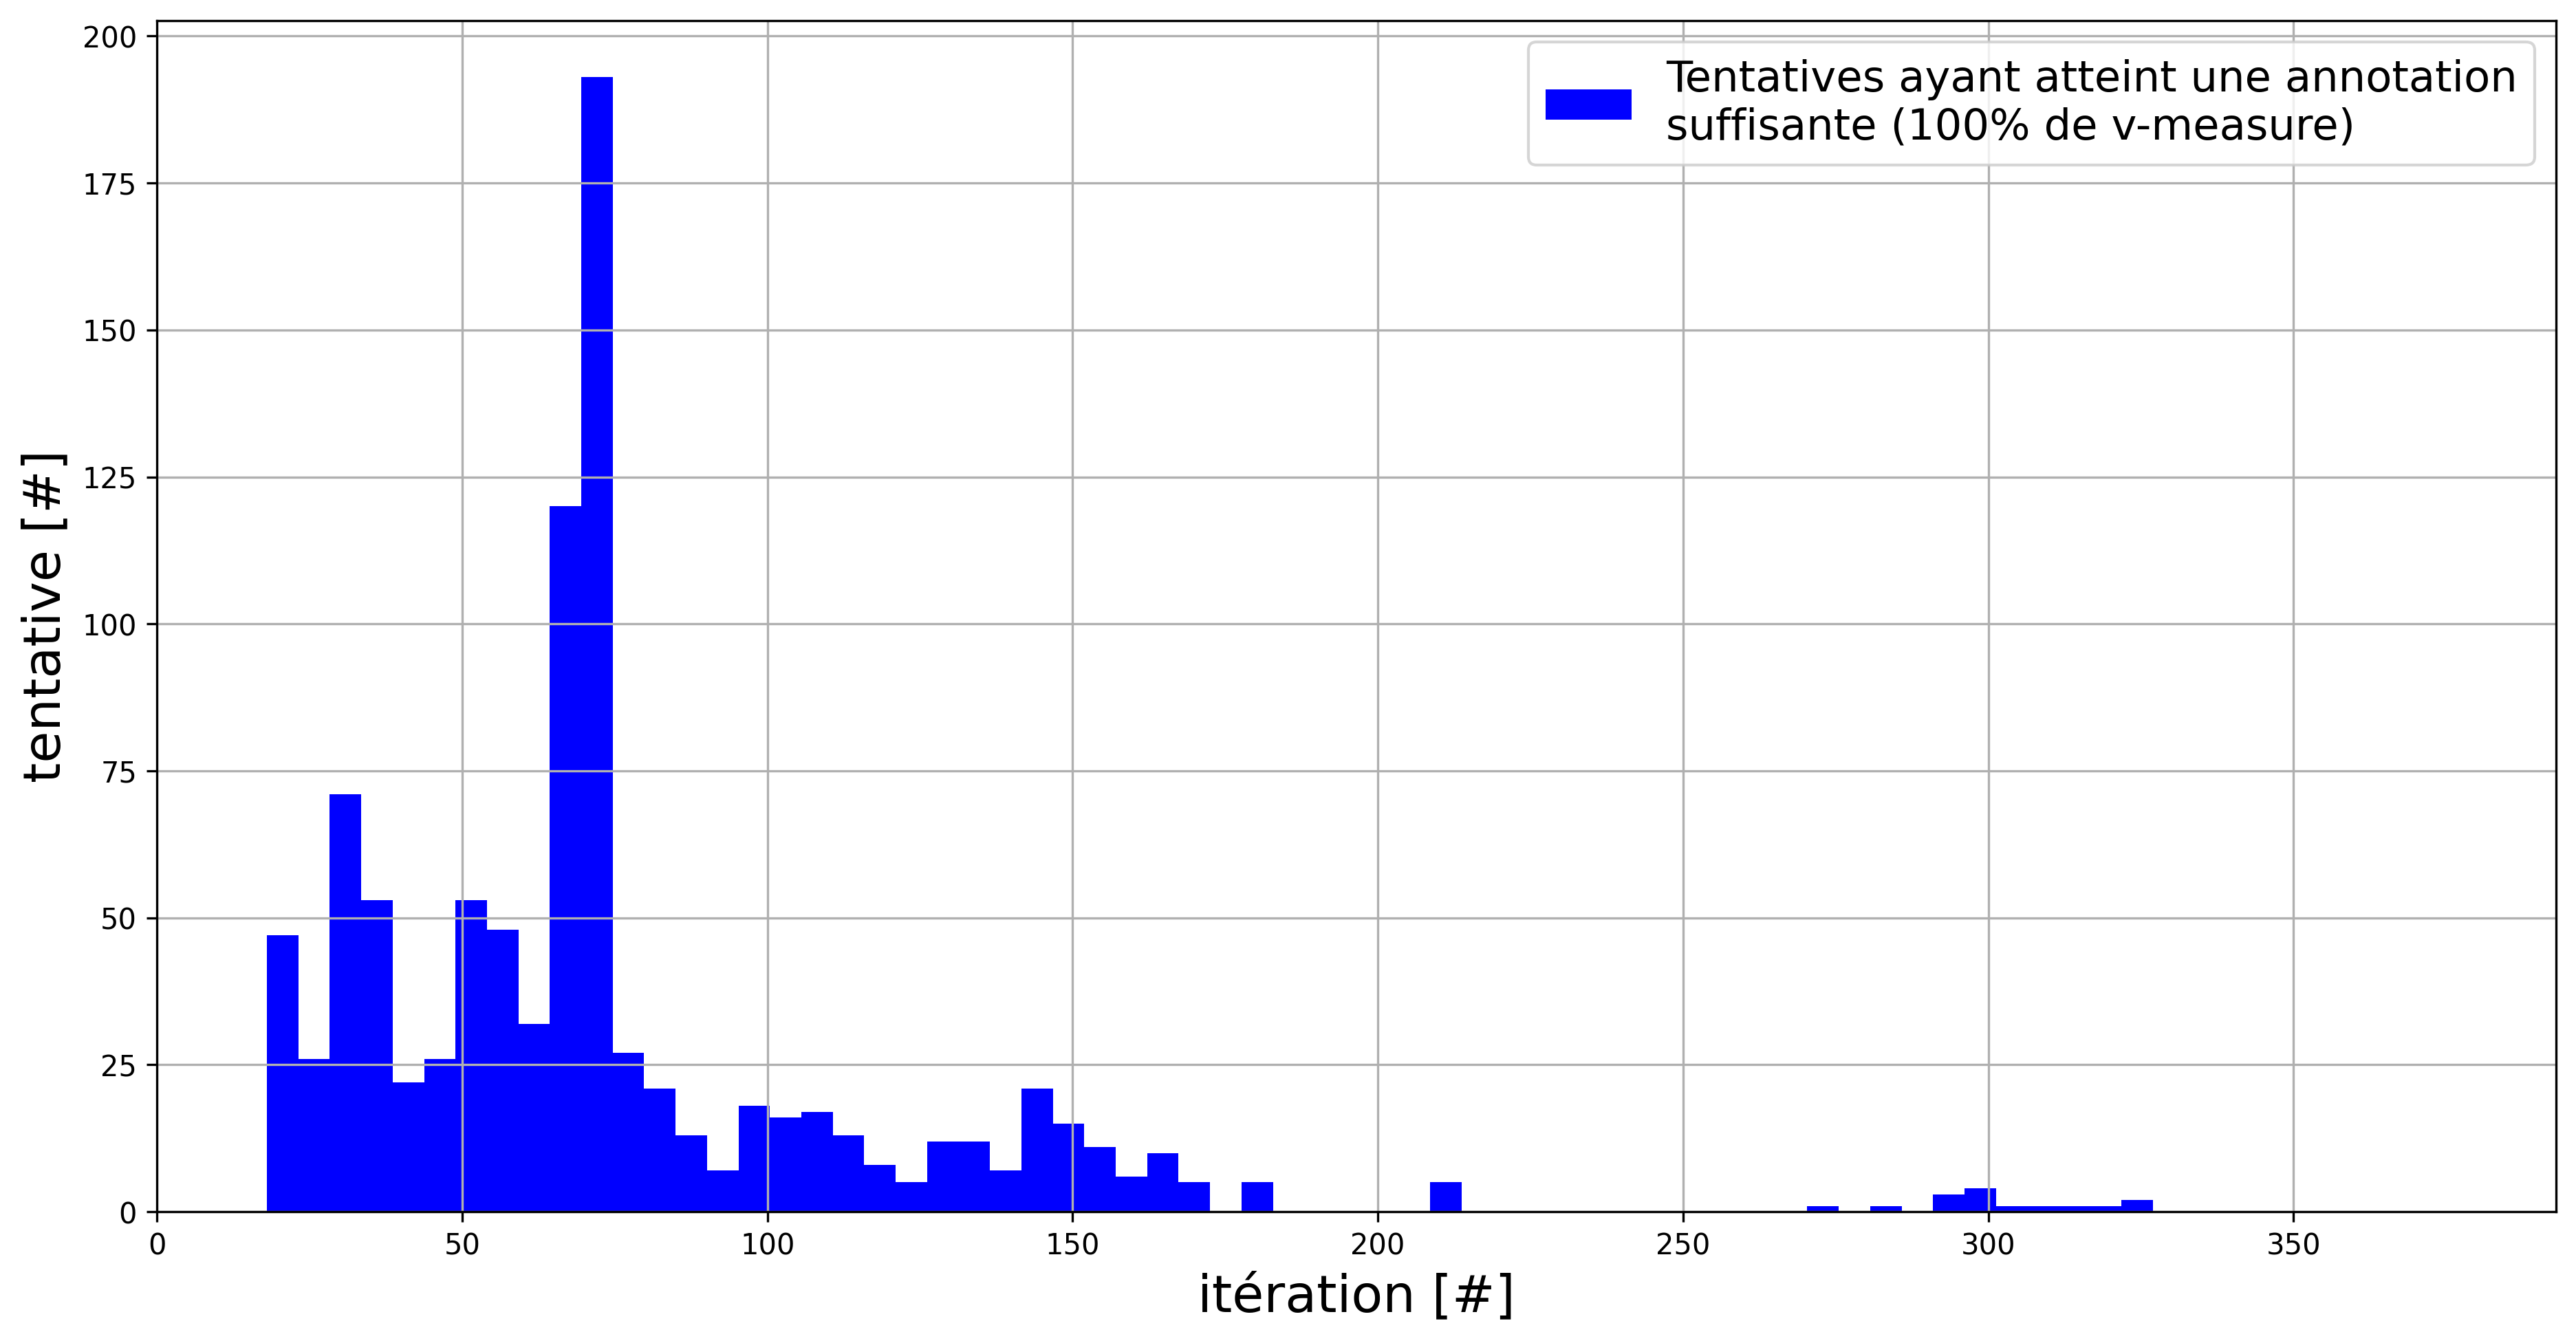
\includegraphics[width=0.90\textwidth]{figures/etude-efficience-histogramme-annotation-suffisante}
				\caption{
					Répartition des tentatives en fonction de l'itération de la méthode à laquelle elles atteignent le seuil d'une annotation suffisante, c'est-à-dire l'itération à laquelle elles parviennent à $100$\% de \texttt{v-measure} entre un résultat obtenu et la vérité terrain.
					L'histogramme est réduit à $60$ pics pour simplifier l'affichage.
				}
				\label{figure:4.2.1-ETUDE-OPTIMISATION-HISTOGRAMME-ANNOTATION-SUFFISANTE}
			\end{figure}
			%
			La \textsc{Table~\ref{table:4.2.1-ETUDE-OPTIMISATION-ANOVA-ANNOTATION-SUFFISANTE}} retranscrit l'influence de chacun des paramètres sur le nombre d'itérations nécessaires pour atteindre une \textbf{annotation suffisante}.
			Les analyses de variance mettent en relief l'effet significatif sur cette convergence du prétraitement (\texttt{eta-carré}: $0.987$, \texttt{p-valeur}: $< 10^{-3}$), de la vectorisation (\texttt{eta-carré}: $0.991$, \texttt{p-valeur}: $< 10^{-3}$), du \textit{clustering} (\texttt{eta-carré}: $0.997$, \texttt{p-valeur}: $< 10^{-3}$) et de l'échantillonnage (\texttt{eta-carré}: $0.998$, \texttt{p-valeur}: $< 10^{-3}$).
			L'analyse post-hoc de ces effets indique que le meilleur paramétrage moyen pour atteindre une \textbf{annotation suffisante} repose sur le prétraitement \texttt{prep.lemma}, le vectorisation \texttt{vect.tfidf}, le \textit{clustering} \texttt{clust.kmeans.cop}, et l'échantillonnage \texttt{samp.closest.diff}. La moyenne du nombre d'itération requis pour ce paramétrage est de $34.60$ (écart-type: $7.44$), soit $1~730$ annotations (écart-type: $372.00$).
			%
			\begin{table}[!htb]
				\begin{center}
				\begin{tabular}{|c|c|c|c|c|c|c|}
					\hline
					% ENTETE DU TABLEAU
					\rowcolor{colorTableHeader!15}
					\multicolumn{2}{|c|}{ \shortstack{Description des \\ facteurs analysés } }
						& \multicolumn{3}{c|}{ \shortstack{ Description statistique \\ des itérations } }
						& \multicolumn{2}{c|}{ \shortstack{ Description des \\ tailles d'effets } }
						\tabularnewline
						\hline
					\rowcolor{colorTableHeader!15}
					Facteur
						& Niveau 
						& Moyenne
						& Rang
						& SE
						& \texttt{ $\eta^{2}$ }
						& \texttt{p-valeur}
						\tabularnewline
						\hline
					
					% PRETRAITEMENT
					\multirow{4}{*}{prétraitement}
						& \texttt{prep.lemma}
						& $72.86$
						& (1)
						& \multirow{4}{*}{ $0.32$ }
						& \multirow{4}{*}{ $0.276$ }
						& \multirow{4}{*}{ \shortstack{ $< 10^{-3}$ \\ ($***$) } }
						\tabularnewline
						\cline{2-4}
						
						& \texttt{prep.simple}
						& $73.30$
						& (2)
						&
						&
						&
						\tabularnewline
						\cline{2-4}
						
						& \texttt{prep.no}
						& $75.24$
						& (2)
						&
						& 
						&
						\tabularnewline
						\cline{2-4}
						
						& \texttt{prep.filter}
						& $83.77$
						& (4)
						&
						&
						&
						\tabularnewline
						\hline
					
					% VECTORISATION
					\multirow{2}{*}{vectorisation}
						& \texttt{vect.tfidf}
						& $71.16$
						& (1)
						& \multirow{2}{*}{ $0.36$ }
						& \multirow{2}{*}{ $0.366$ }
						& \multirow{2}{*}{ \shortstack{$< 10^{-3}$ \\ ($***$)} }
						\tabularnewline
						\cline{2-4}
						
						& \texttt{vect.frcorenewsmd}
						& $81.43$
						& (2)
						&
						&
						&
						\tabularnewline
						\hline
					
					% CLUSTERING
					\multirow{6}{*}{clustering}
						& \texttt{clust.kmeans.cop}
						& $62.23$
						& (1)
						& \multirow{6}{*}{ $0.42$ }
						& \multirow{6}{*}{ $0.700$ }
						& \multirow{6}{*}{ \shortstack{$< 10^{-3}$ \\ ($***$)} }
						\tabularnewline
						\cline{2-4}
						
						& \texttt{clust.hier.avg}
						& $65.13$
						& (2)
						&
						&
						&
						\tabularnewline
						\cline{2-4}
						
						& \texttt{clust.hier.sing}
						& $75.44$
						& (3)
						&
						& 
						&
						\tabularnewline
						\cline{2-4}
						
						& \texttt{clust.hier.ward}
						& $80.44$
						& (4)
						&
						& 
						&
						\tabularnewline
						\cline{2-4}
						
						& \texttt{clust.hier.comp}
						& $81.46$
						& (5)
						&
						&
						&
						\tabularnewline
						\cline{2-4}
						
						& \texttt{clust.spec}
						& $93.06$
						& (6)
						&
						& 
						&
						\tabularnewline
						\hline
					
					% ECHANTILLONNAGE
					\multirow{4}{*}{échantillonnage}
						& \texttt{samp.closest.diff}
						& $50.29$
						& (1)
						& \multirow{4}{*}{ $0.39$ }
						& \multirow{4}{*}{ $0.950$ }
						& \multirow{4}{*}{ \shortstack{$< 10^{-3}$ \\ ($***$)} }
						\tabularnewline
						\cline{2-4}
						
						& \texttt{samp.random.same}
						& $56.38$
						& (2)
						&
						&
						&
						\tabularnewline
						\cline{2-4}
						
						& \texttt{samp.random.full}
						& $71.95$
						& (3)
						&
						& 
						&
						\tabularnewline
						\cline{2-4}
						
						& \texttt{samp.farhtest.same}
						& $126.55$
						& (4)
						&
						&
						&
						\tabularnewline
						\hline
				\end{tabular}
				\end{center}
				\caption{
					ANOVA du nombre d'itérations nécessaires pour l'obtention de $100$\% de v-mesure. Les ($\textit{*}$) dénotent le niveau de significativité ($\alpha=0.05$). Pour les effets significatifs, les chiffres précisés entre parenthèses dans la colonne \texttt{Moyenne} indiquent le classement des niveaux selon les analyses post-hoc.
				}
				\label{table:4.2.1-ETUDE-OPTIMISATION-ANOVA-ANNOTATION-SUFFISANTE}
			\end{table}
			
			%%% Analyse d'une annotation exhaustive.
			Enfin, pour avoir une \textbf{annotation exhaustive} (\textit{annoter toutes les contraintes possibles}), la moyenne des itérations est de $88.98$ (min: $20$, max: $394$, écart-type: $68.21$), soit une moyenne de $4~431.34$ annotations (min: $1~000$, max: $19~656$, écart-type: $3~405.16$).
			La \textsc{Figure~\ref{figure:4.2.1-ETUDE-OPTIMISATION-HISTOGRAMME-ANNOTATION-EXHAUSTIVE}} représente la répartition de ces itérations au cours des différentes tentatives.
			On peut noter les deux cas intéressants suivants :
			\begin{itemize}
				\item[$\bullet$] Les tentatives les plus rapides furent celles avec un prétraitement des données \texttt{prep.no} ou \texttt{prep.lemma}, une vectorisation des données \texttt{vect.tfidf}, un algorithme de \textit{clustering} sous contraintes \texttt{clust.hier.comp} ou \texttt{clust.hier.ward}, et un échantillonnage de contraintes \texttt{samp.closest.diff}. Ces tentatives ont requis $20$ itérations, soit $1~000$ annotations, dont $653$ (respectivement $668$) contraintes \texttt{MUST-LINK}.
				\item[$\bullet$] Les tentatives les plus lentes furent celles avec un prétraitement des données \texttt{prep.simple}, une vectorisation des données \texttt{vect.frcorenewsmd}, un \textit{clustering} \texttt{clust.hier.sing}, et un échantillonnage de contraintes \texttt{samp.closest.diff}. Ces tentatives ont requis $394$ itérations, soit $19~656$ annotations, dont $682$ contraintes \texttt{MUST-LINK}.
			\end{itemize}
			%
			\begin{figure}[!htb]
				\centering
				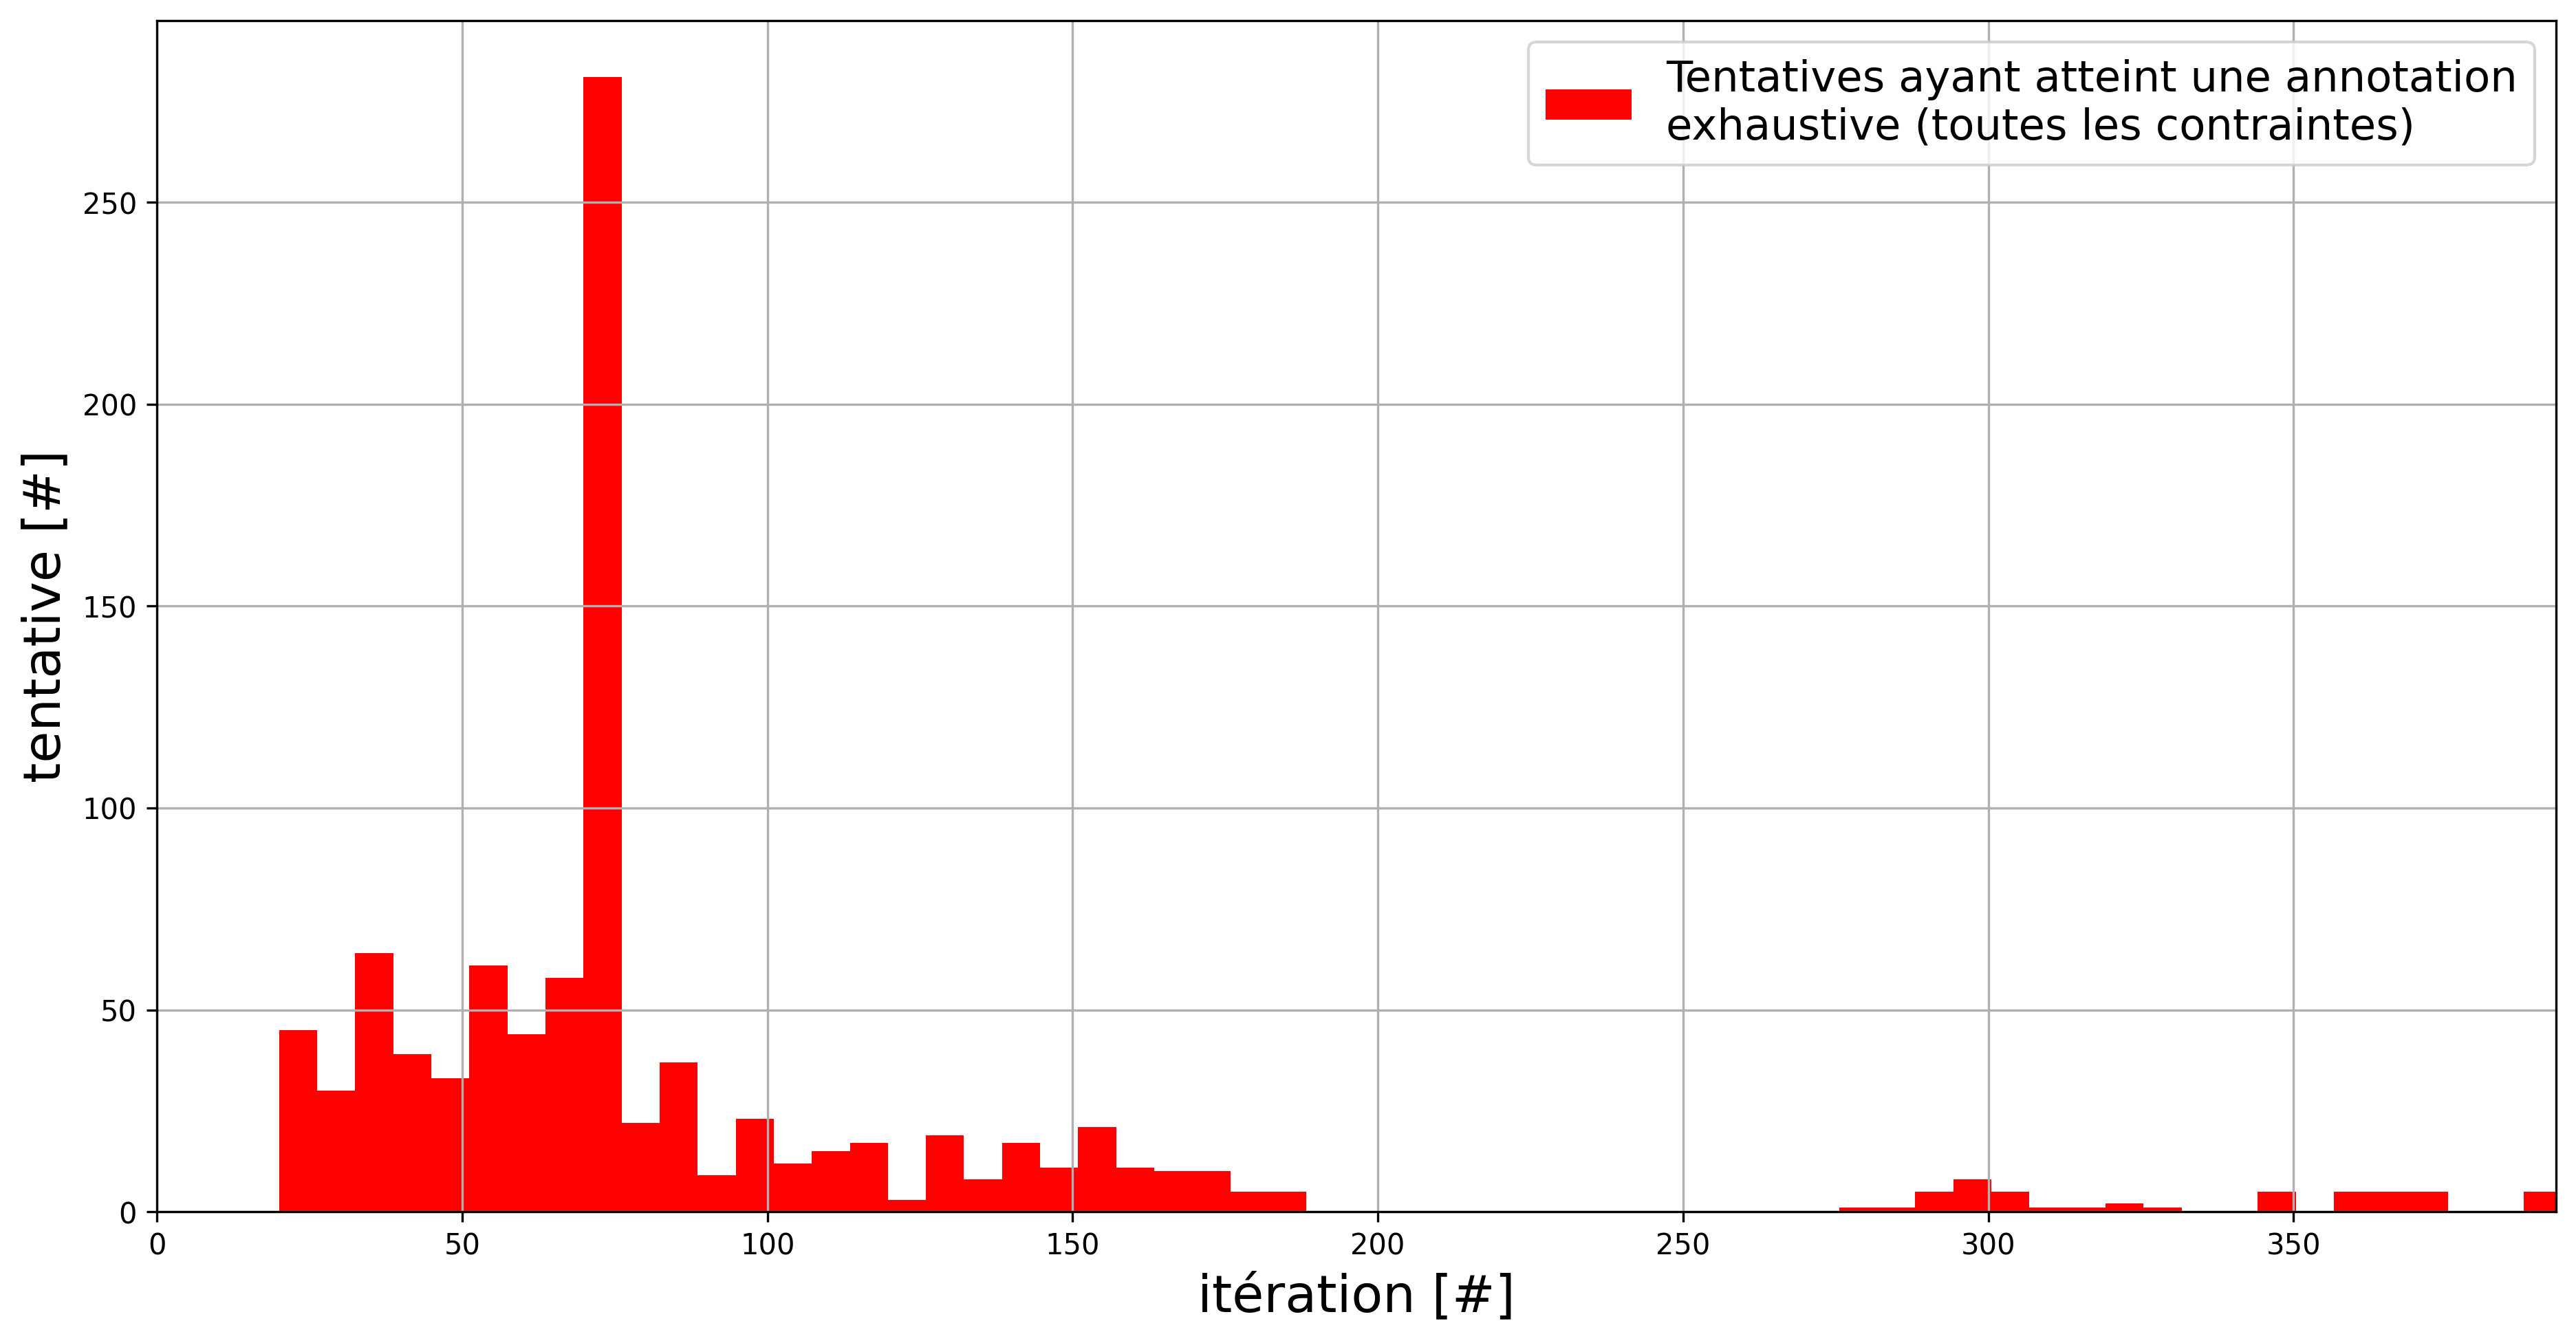
\includegraphics[width=0.90\textwidth]{figures/etude-efficience-histogramme-annotation-exhaustive}
				\caption{
					Répartition des tentatives en fonction de l'itération de la méthode à laquelle elles atteignent le seuil d'une annotation exhaustive, c'est-à-dire l'itération à laquelle toutes les contraintes possibles entre les données ont été annotées.
					L'histogramme est réduit à $60$ pics pour simplifier l'affichage.
				}
				\label{figure:4.2.1-ETUDE-OPTIMISATION-HISTOGRAMME-ANNOTATION-EXHAUSTIVE}
			\end{figure}
			%
			La \textsc{Table~\ref{table:4.2.1-ETUDE-OPTIMISATION-ANOVA-ANNOTATION-EXHAUSTIVE}} retranscrit l'influence de chacun des paramètres sur le nombre d'itérations nécessaires pour atteindre une \textbf{annotation exhaustive}.
			Les analyses de variance mettent en relief l'effet significatif sur cette convergence du prétraitement (\texttt{eta-carré}: $0.909$, \texttt{p-valeur}: $< 10^{-3}$), de la vectorisation (\texttt{eta-carré}: $0.985$, \texttt{p-valeur}: $< 10^{-3}$), du \textit{clustering} (\texttt{eta-carré}: $0.999$, \texttt{p-valeur}: $< 10^{-3}$) et de l'échantillonnage (\texttt{eta-carré}: $0.997$, \texttt{p-valeur}: $< 10^{-3}$).
			L'analyse post-hoc de ces effets indique que le meilleur paramétrage moyen pour atteindre une \textbf{annotation exhaustive} repose sur le prétraitement \texttt{prep.lemma}, le vectorisation \texttt{vect.tfidf}, le \textit{clustering} \texttt{clust.kmeans.cop}, et l'échantillonnage \texttt{samp.random.same}. La moyenne du nombre d'itération requis pour ce paramétrage est de $32.60$ (écart-type: $1.14$), soit $1~630$ annotations (écart-type: $57.00$).
			%
			\begin{table}[!htb]
				\begin{center}
				\begin{tabular}{|c|c|c|c|c|c|c|}
					\hline
					% ENTETE DU TABLEAU
					\rowcolor{colorTableHeader!15}
					\multicolumn{2}{|c|}{ \shortstack{Description des \\ facteurs analysés } }
						& \multicolumn{3}{c|}{ \shortstack{ Description statistique \\ des itérations } }
						& \multicolumn{2}{c|}{ \shortstack{ Description des \\ tailles d'effets } }
						\tabularnewline
						\hline
					\rowcolor{colorTableHeader!15}
					Facteur
						& Niveau 
						& Moyenne
						& Rang
						& SE
						& \texttt{ $\eta^{2}$ }
						& \texttt{p-valeur}
						\tabularnewline
						\hline
					
					% PRETRAITEMENT
					\multirow{4}{*}{prétraitement}
						& \texttt{prep.lemma}
						& $85.89$
						& (1)
						& \multirow{4}{*}{ $0.42$ }
						& \multirow{4}{*}{ $0.052$ }
						& \multirow{4}{*}{ \shortstack{$< 10^{-3}$ \\ ($***$)} }
						\tabularnewline
						\cline{2-4}
						
						& \texttt{prep.filter}
						& $89.55$
						& (2)
						&
						&
						&
						\tabularnewline
						\cline{2-4}
						
						& \texttt{prep.simple}
						& $89.64$
						& (2)
						&
						& 
						&
						\tabularnewline
						\cline{2-4}
						
						& \texttt{prep.no}
						& $90.81$
						& (4)
						&
						&
						&
						\tabularnewline
						\hline
					
					% VECTORISATION
					\multirow{2}{*}{vectorisation}
						& \texttt{vect.tfidf}
						& $85.50$
						& (1)
						& \multirow{2}{*}{ $0.39$ }
						& \multirow{2}{*}{ $0.165$ }
						& \multirow{2}{*}{ \shortstack{$< 10^{-3}$ \\ ($***$)} }
						\tabularnewline
						\cline{2-4}
						
						& \texttt{vect.frcorenewsmd}
						& $92.46$
						& (2)
						&
						&
						&
						\tabularnewline
						\hline
					
					% CLUSTERING
					\multirow{6}{*}{clustering}
						& \texttt{clust.kmeans.cop}
						& $64.99$
						& (1)
						& \multirow{6}{*}{ $0.39$ }
						& \multirow{6}{*}{ $0.894$ }
						& \multirow{6}{*}{ \shortstack{$< 10^{-3}$ \\ ($***$)} }
						\tabularnewline
						\cline{2-4}
						
						& \texttt{clust.hier.avg}
						& $78.54$
						& (2)
						&
						&
						&
						\tabularnewline
						\cline{2-4}
						
						& \texttt{clust.hier.ward}
						& $81.31$
						& (3)
						&
						& 
						&
						\tabularnewline
						\cline{2-4}
						
						& \texttt{clust.hier.comp}
						& $82.49$
						& (3)
						&
						& 
						&
						\tabularnewline
						\cline{2-4}
						
						& \texttt{clust.spec}
						& $93.78$
						& (5)
						&
						&
						&
						\tabularnewline
						\cline{2-4}
						
						& \texttt{clust.hier.comp}
						& $132.75$
						& (6)
						&
						& 
						&
						\tabularnewline
						\hline
					
					% ECHANTILLONNAGE
					\multirow{4}{*}{échantillonnage}
						& \texttt{samp.random.same}
						& $57.23$
						& (1)
						& \multirow{4}{*}{ $0.42$ }
						& \multirow{4}{*}{ $0.930$ }
						& \multirow{4}{*}{ \shortstack{$< 10^{-3}$ \\ ($***$)} }
						\tabularnewline
						\cline{2-4}
						
						& \texttt{samp.random.full}
						& $72.80$
						& (2)
						&
						&
						&
						\tabularnewline
						\cline{2-4}
						
						& \texttt{samp.closest.diff}
						& $98.38$
						& (3)
						&
						& 
						&
						\tabularnewline
						\cline{2-4}
						
						& \texttt{samp.farhtest.same}
						& $132.75$
						& (4)
						&
						&
						&
						\tabularnewline
						\hline
				\end{tabular}
				\end{center}
				\caption{
					ANOVA du nombre d'itérations nécessaires pour annoter toutes les contraintes possibles. Les ($\textit{*}$) dénotent le niveau de significativité ($\alpha=0.05$). Pour les effets significatifs, les chiffres précisés entre parenthèses dans la colonne \texttt{Moyenne} indiquent le classement des niveaux selon les analyses post-hoc.
				}
				\label{table:4.2.1-ETUDE-OPTIMISATION-ANOVA-ANNOTATION-EXHAUSTIVE}
			\end{table}
		
		
			% Graphe d'évolution de la v-measure moyenne, min et max.
			La \textsc{Figure~\ref{figure:4.2.1-ETUDE-OPTIMISATION-EVOLUTION-PAR-FACTEURS}} représente les évolutions moyennes de la \texttt{v-measure} du \textit{clustering} en fonction du nombre d'itération de la méthode pour les différentes valeurs des facteurs analysés (prétraitement en haut à gauche, vectorisation en haut à droite, \textit{clustering} en bas à gauche, échantillonnage en bas à droite).
			La \textsc{Figure~\ref{figure:4.2.1-ETUDE-OPTIMISATION-EVOLUTION-MEILLEUR-PARAMETRAGE}} représente cette même évolution pour les meilleurs paramétrages moyens destinés à atteindre les trois seuils d'annotation définis (partiel, suffisant, exhaustif), où nous y constatons une baisse significative du nombre d'itérations nécessaire à la convergence par rapport à la moyenne des tentatives.
			%
			\begin{figure}[!htb]
				\centering
				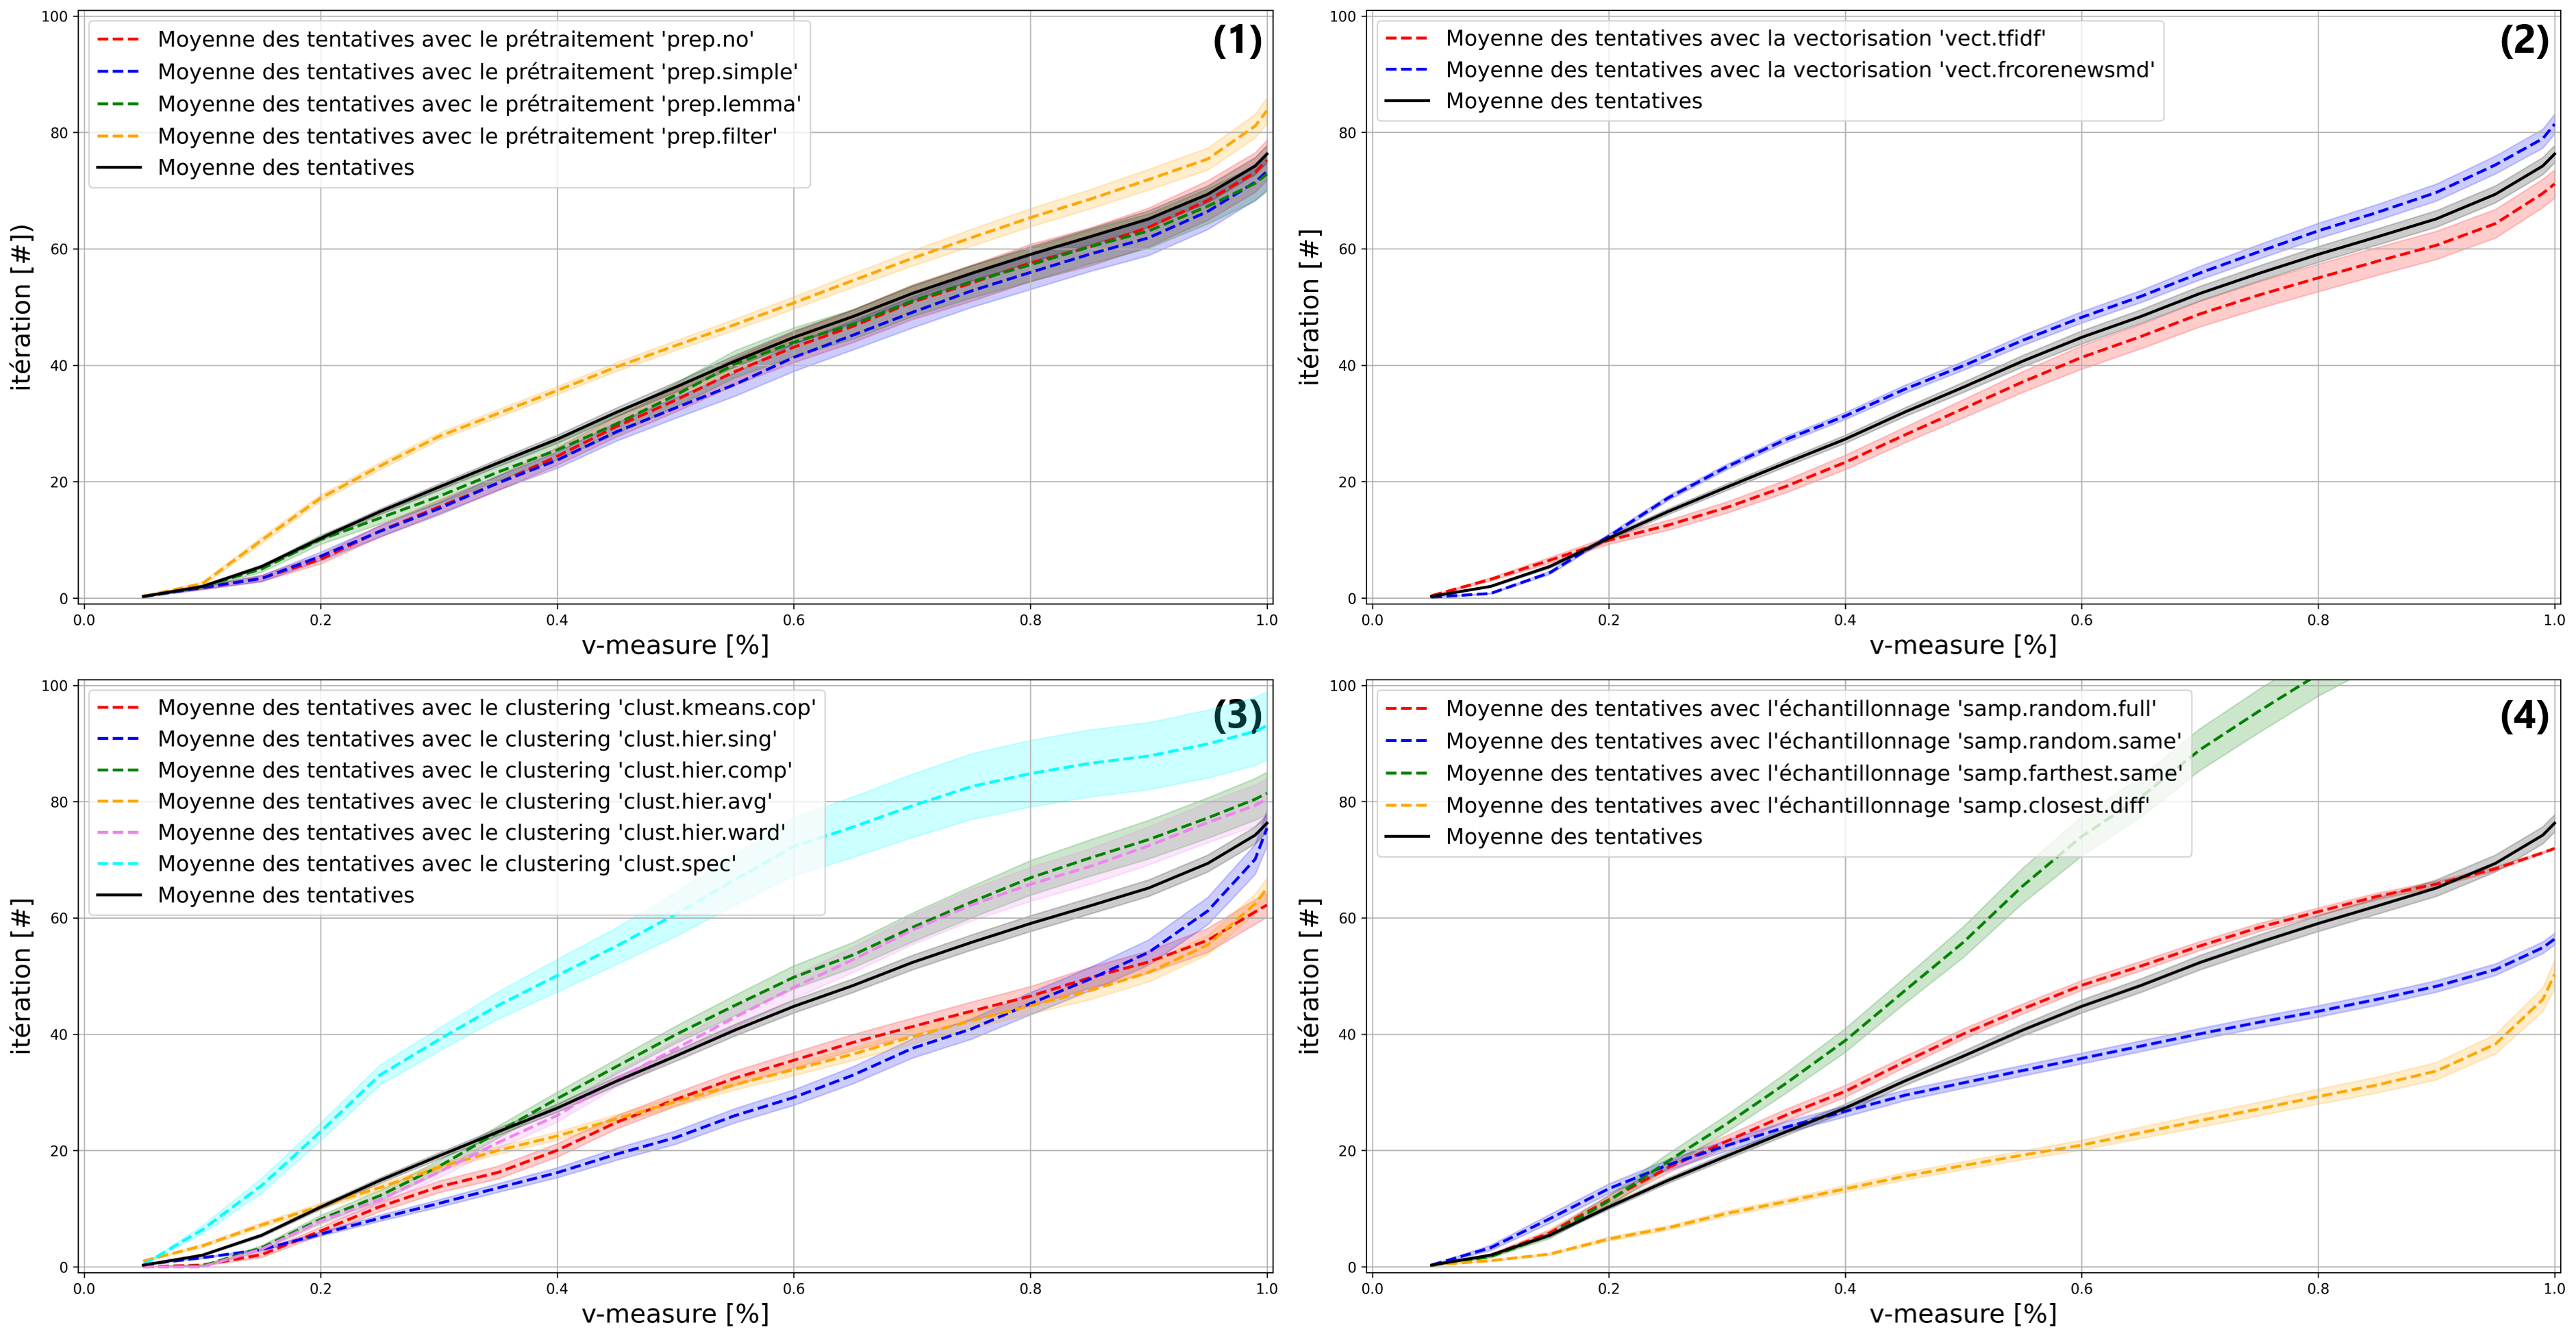
\includegraphics[width=0.95\textwidth]{figures/etude-efficience-evolution-moyenne-par-vmeasure-par-facteur}
				\caption{Évolution des moyennes du nombre d'itérations nécessaire de la méthode de \textit{clustering} interactif pour obtenir un seuil défini de \texttt{v-measure} entre un résultat obtenu et la vérité terrain, moyennes réalisées sur les différentes valeurs que peuvent prendre les facteurs analysés et affichées par facteur : \textbf{(1)} prétraitement, \textbf{(2)} vectorisation, \textbf{(3)} \textit{clustering} et \textbf{(4)} échantillonnage. \\
				Note : \textit{Le seuil d'annotation exhaustive (annoter toutes les contraintes possibles) n'étant pas exprimé en terme de \texttt{v-measure}, ce seuil n'est pas affiché ici.}}
				\label{figure:4.2.1-ETUDE-OPTIMISATION-EVOLUTION-PAR-FACTEURS}
			\end{figure}
			%
			\begin{figure}[!htb]
				\centering
				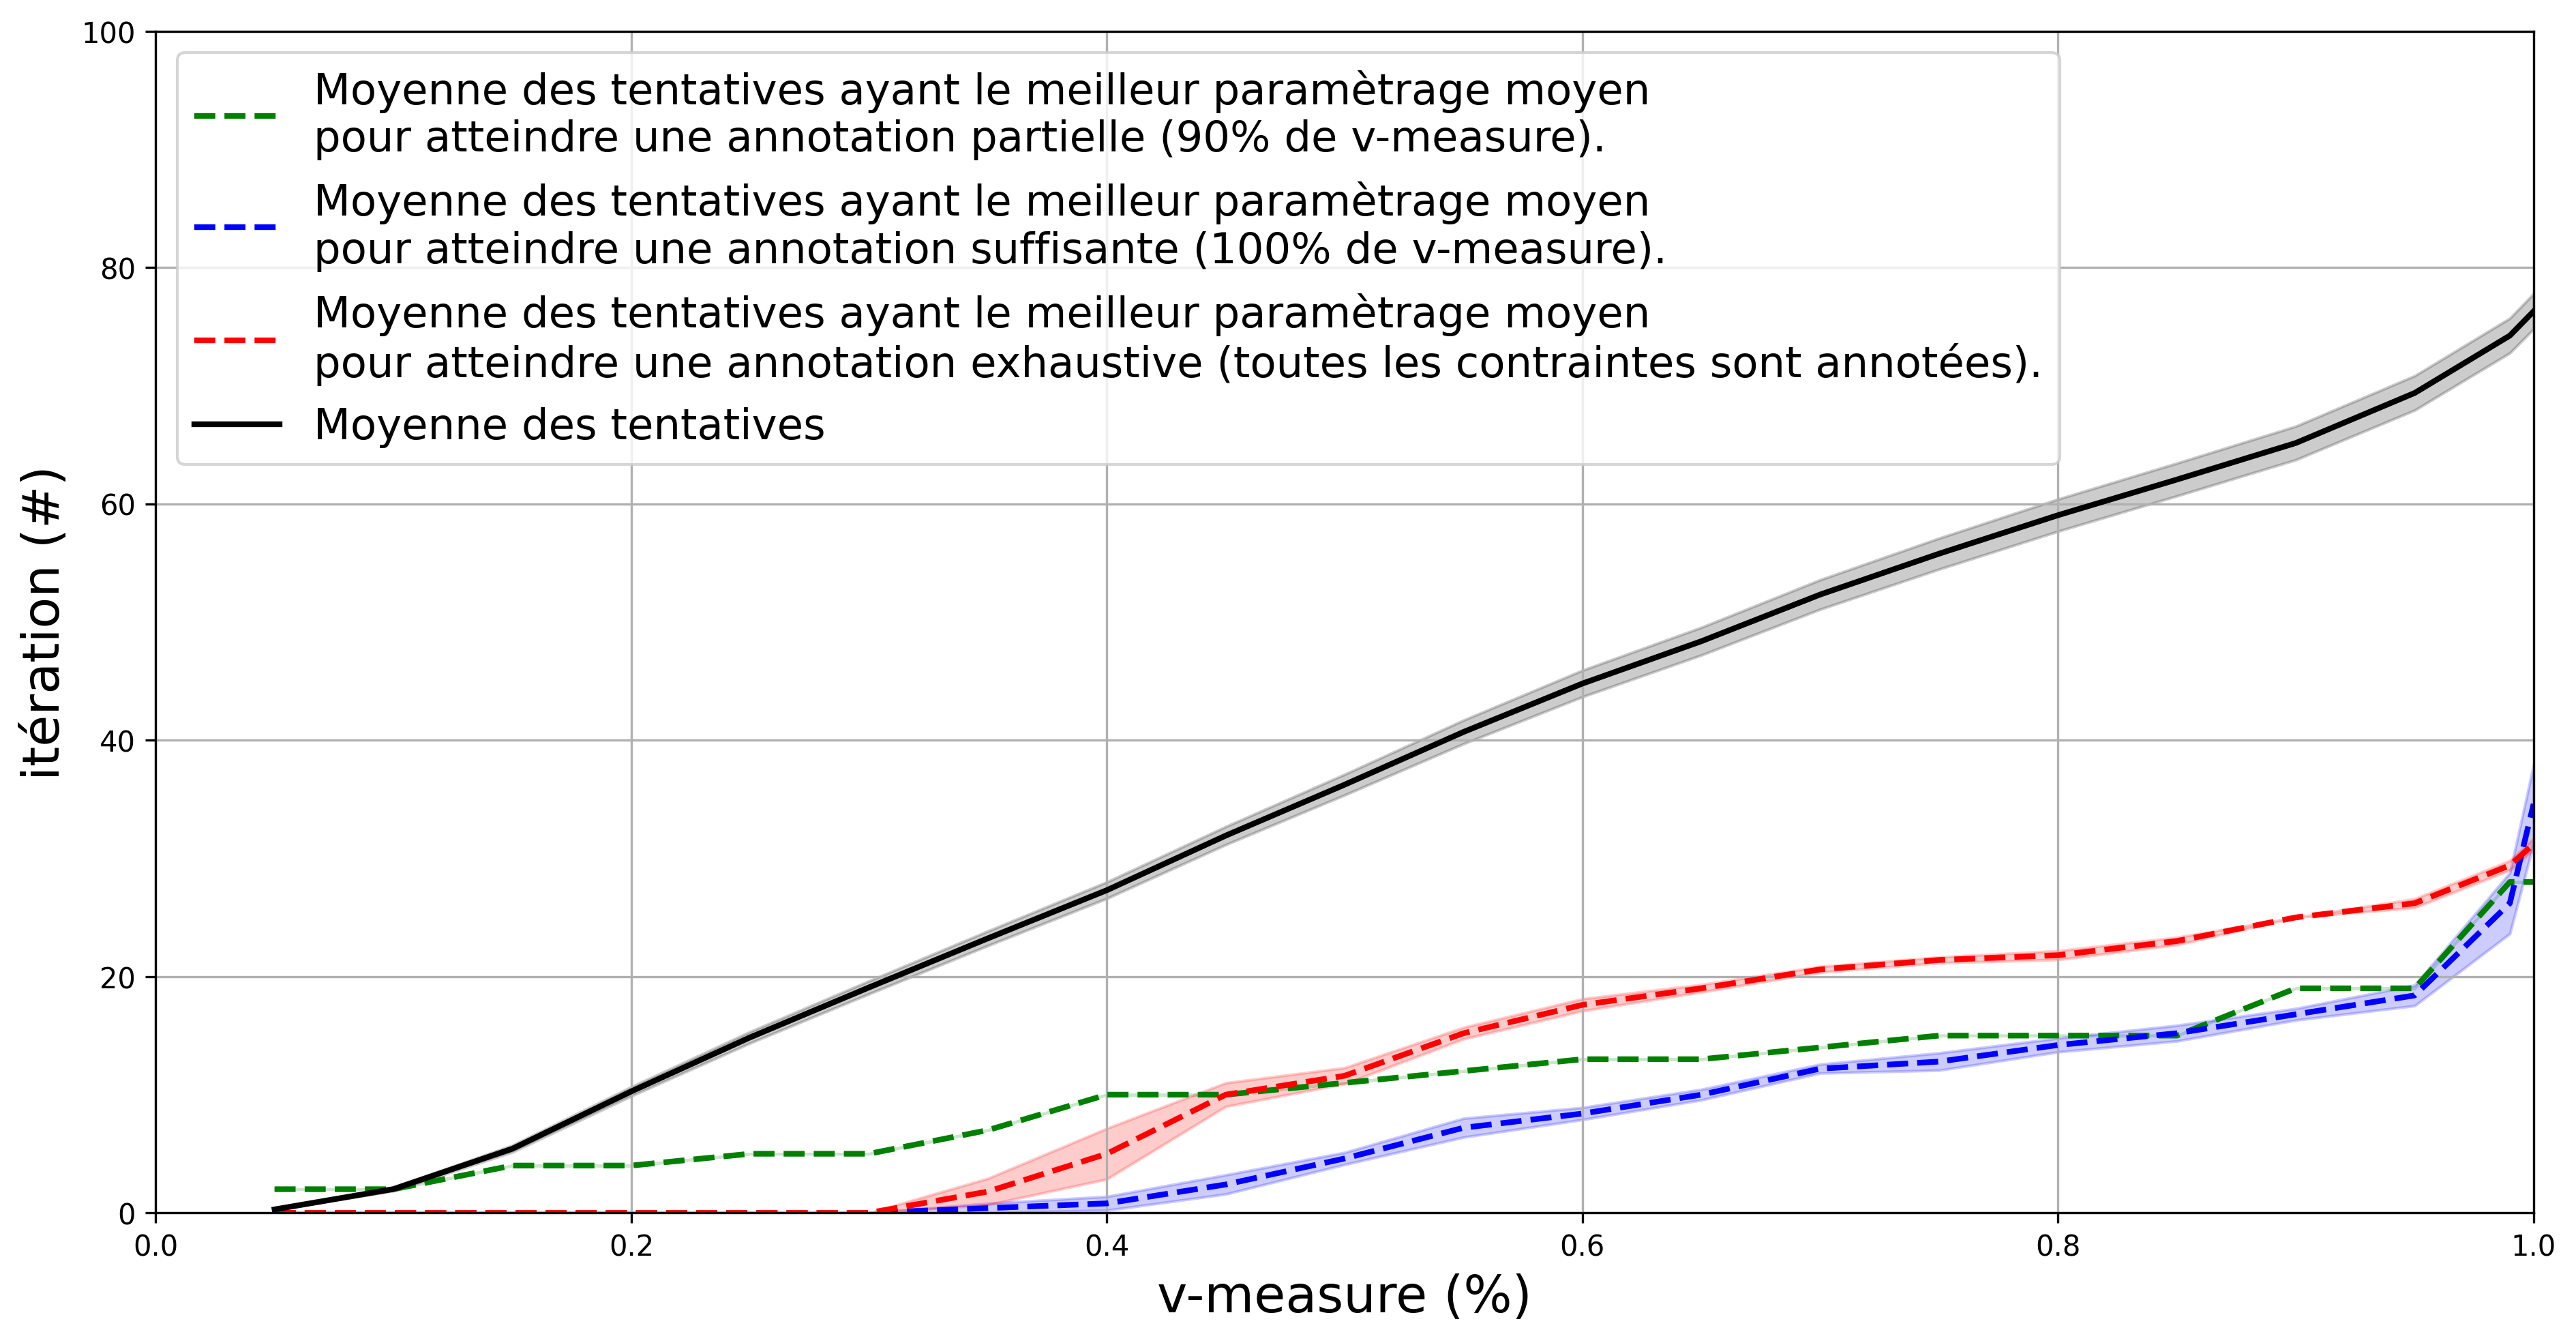
\includegraphics[width=0.95\textwidth]{figures/etude-efficience-evolution-moyenne-5best-par-vmeasure}
				\caption{
					Évolution des moyennes du nombre d'itérations nécessaire de la méthode de \textit{clustering} interactif pour obtenir un seuil défini de \texttt{v-measure} entre un résultat obtenu et la vérité terrain, moyennes réalisées sur les différentes seuils d'annotations étudiés : l'annotation partielle (\textit{atteindre une \texttt{v-measure} de $90$\%}), l'annotation suffisante (\textit{atteindre une \texttt{v-measure} de $100$\%}) et l'annotation exhaustive (\textit{annoter toutes les contraintes possibles}).
				}
				\label{figure:4.2.1-ETUDE-OPTIMISATION-EVOLUTION-MEILLEUR-PARAMETRAGE}
			\end{figure}

		%%% Discussion.
		\subsubsection{Discussion}

			% Rappel de l'objectif : être efficient.
			L'objectif de l'étude est de trouver une implémentation "efficiente" du \textit{clustering} interactif permettant d'obtenir une base d'apprentissage correctement annotée en un minimum d'annotation.
			Pour trouver si une telle implémentation existe et quels en sont les paramètres optimaux, nous avons analysé l'impact de différentes paramétrages sur les tâches principales de la méthode (\textbf{prétraitement}, \textbf{vectorisation}, \textbf{clustering sous contraintes}, \textbf{échantillonnage}) en nous basant sur des simulations d'annotation d'un jeu de données.
			\\
			
			% Première remarque : Choix d'un seuil à 90\% de v-measure.
			Dans l'optique d'être efficient, nous excluons le désir d'annoter \textbf{exhaustivement} le jeu de données car la charge de travail estimée est trop importante.
			(cf. discussion de la \textsc{Section~\ref{section:4.1-HYPOTHESE-EFFICACITE}} (hypothèse d'efficacité))
			Nous préférons donc nous concentrer sur deux seuils d'annotation plus réalistes : celui d'une \textbf{annotation partielle} (atteindre $90$\% de \texttt{v-measure} avec la vérité terrain) et celui d'une \textbf{annotation suffisante} (atteindre $100$\% de \texttt{v-measure} avec la vérité terrain en un minimum de contraintes). 
			
			% Meilleur paramétrage.
			L'étude réalisée met en avant l'impact significatif des quatre tâches principales (\textbf{prétraitement}, \textbf{vectorisation}, \textbf{\textit{clustering} sous contraintes}, \textbf{échantillonnage}) sur la vitesse de convergence de la méthode pour atteindre les seuils définis de $90$\% et $100$\% de \texttt{v-measure}. Il existe donc bien un paramétrage permettant d'optimiser l'implémentation proposée et de réduire le nombre de contraintes nécessaires à annoter :
			\begin{enumerate}
				% Annotation partielle.
				\item pour une \textbf{annotation partielle} ($90$\% de \texttt{v-measure}), le meilleur paramétrage moyen est constitué du prétraitement simple (\texttt{prep.simple}), de la vectorisation TF-IDF (\texttt{vect.tfidf}), du \textit{clustering} hiérarchique à lien moyen (\texttt{clust.hier.avg}) et de l'échantillonnage des données les plus proches dans des clusters différents (\texttt{sampl.closest.diff}).
				Avec ce paramétrage, il faut en moyenne $950$ annotations de contraintes pour obtenir une \texttt{v-measure} de $90$\% ;
				% Annotation suffisante.
				\item pour une \textbf{annotation suffisante} ($100$\% de \texttt{v-measure}), le meilleur paramétrage moyen est constitué du prétraitement avec lemmatisation (\texttt{prep.lemma}), de la vectorisation TF-IDF (\texttt{vect.tfidf}), du \textit{clustering} KMeans avec modèle COP (\texttt{clust.kmeans.cop}) et de l'échantillonnage des données les plus proches dans des clusters différents (\texttt{sampl.closest.diff}).
				Avec ce paramétrage, il faut en moyenne $1~750$ annotations de contraintes pour obtenir une \texttt{v-measure} de $100$\% ;
				% Annotation exhaustive.
				\item le cas d'une \textbf{annotation exhaustive} (annoter toutes les contraintes possibles sur les données) n'est pas explicité ici mais peut se déduire des résultats décrits plus haut.
			\end{enumerate}
			%
			\begin{leftBarAuthorOpinion}
				% Prétraitement et Vectorisation.
				On note que les facteurs de prétraitement et de vectorisation sont significatifs possèdent toutefois de faibles valeurs de variance expliquée ($\eta^{2} < 0.40$).
				
				% Echantillonnage et Clustering.
				Les facteurs de \textit{clustering} et d'échantillonnage ont quand à eux des valeurs plus fortes ($\eta^{2} > 0.70$), dénotant ainsi un plus grand pouvoir explicatif de la variance des résultats.
				Notre attention s'attarde particulièrement sur l'échantillonnage des données les plus proches dans des clusters différents (\texttt{sampl.closest.diff}) qui s'avère très prometteur : cette sélection semble permettre de corriger efficacement la frontière des \textit{clusters} en favorisant l'ajout de contraintes \texttt{MUST-LINK} sur des données séparées à tord.
				Or les corrections introduisant des contraintes \texttt{MUST-LINK} sont plus explicites que les contraintes \texttt{CANNOT-LINK} dont l'utilisation est plus ambiguë (\textit{dans le premier cas, on sait que les deux données sont désormais à mettre dans le même \textit{cluster} ; dans le second, ont sait qu'il faut séparer les deux données sans exprimer dans quels \textit{clusters} ils doivent aller}).
				Ainsi, nous sommes d'avis que l'échantillonnage \texttt{sampl.closest.diff} est efficiente car elle permet d'introduire efficacement des contraintes dont l'utilité est immédiate pour corriger le \textit{clustering}.
			\end{leftBarAuthorOpinion}

			%%% Avantages.
			Ainsi, cette étude permet de répondre à la limite du nombre de contraintes requis (discutée dans l'hypothèse d'efficacité, \textsc{Section~\ref{section:4.1-HYPOTHESE-EFFICACITE}}).
			%%% Avantage 1: Optimisation du nombre de contraintes.
			En effet, l'optimisation des paramètres de l'implémentation du \textit{clustering} interactif permet de réduire considérablement le nombre de contraintes nécessaires pour obtenir une base d'apprentissage exploitable.
			En nous basant sur la \textsc{Table~\ref{table:4.1.1-ETUDE-CONVERGENCE-EVOLUTION}} de l'étude de convergence, et dans le cadre de l'annotation d'un jeu de $500$ données, nous sommes passé d'un paramétrage moyen nécessitant $3~750$ (respectivement $10~000$) contraintes à un paramétrage optimisé ne nécessitant que $950$ (respectivement $1~750$) contraintes pour atteindre un seuil de $90$\% (respectivement $100$\%) \texttt{v-measure}.
			L'ordre de grandeur de la charge de travail demandée aux annotateurs est donc située entre $2$ et $4$ fois la taille du jeu de données.
			
			% Avantage 2: La méthode devient réaliste !
			Cette estimation est plus raisonnable que celle réalisée en \textsc{Section~\ref{section:4.1-HYPOTHESE-EFFICACITE}}.
			De plus, en considérant que les annotations sont binaires et demandent a priori une charge mental plus faible que les annotations par attribution de label ("\textit{les données sont-elles similaires ?}" vs "\textit{quel est l'étiquette de cette donnée ?}", cf. \cite{hart-staveland:1988:development-nasatlx-task}), nous pouvons espérer que la charge totale nécessaire à l'annotation avec une méthodologie basée sur le \textit{clustering} interactif est comparable à celles des méthodes traditionnelles.
			Nous confirmerons cette conclusion en étudiant le temps nécessaire à un opérateur pour annoter un lot de contraintes (cf. \textsc{Section~\ref{section:4.3.1-ETUDE-COUTS-TEMPS-ANNOTATION}}).
			\\
			
			%%% Limites.
			Afin de compléter cette analyse d'efficience, quelques pistes sont encore à explorer.
			
			% Limite 1 : Coût temporel.
			D'une part, une étude de coût est à réaliser pour trancher le choix de paramètre optimaux réalistes.
			En effet, il est intéressant d'étudier le coût machine (temps CPU utilisé) et le coût humain (temps d'annotation) afin d'affiner les choix techniques et de compléter les arguments sur l'utilisation en situation réelle d'une méthodologie d'annotation basée sur le \textit{clustering} interactif.
			Cette étude sera l'occasion de rentrer en détail dans la comparaison de la charge demander à l'annotateur, tant sur la durée que sur la complexité de la tâche d'annotation.
			Cet aspect sera traité dans la \textsc{Section~\ref{section:4.3-HYPOTHESE-COUTS}} (hypothèse des coûts).
			
			% Limite 2 : Valeur métier de ce 90\% (pas de vérité terrain en pratique).
			D'autre part, l'étude réalisée se base sur des seuils de performance par rapport à une vérité terrain.
			Or en situation réelle, cette comparaison avec la vérité terrain n'est pas possible car elle est précisément en cours de conception (la base d'apprentissage finale devant être la vérité terrain).
			De plus, un tel score n'est pas le plus explicite pour pour un expert métier pour qui un score de \texttt{v-measure} n'est pas révélateur de la pertinence métier de la segmentation proposée des données.
			Dans un registre similaire, il est possible que l'évolution du partitionnement des données passe par plusieurs états stables et pertinents, mais que l'annotateur soit obligé d'affiner sa vision en annotant certaines contraintes ambiguës.
			Cela peut être la cas avec des \textit{clusters} traitant en fin de compte de sujets très similaires (\textit{ajouter des \texttt{MUST-LINK} pour les fusionner}) ou avec un \textit{cluster} qui regroupe finalement plusieurs thématiques (\textit{ajouter des \texttt{CANNOT-LINK} pour le segmenter})
			Il manque donc une stratégie d'évaluation de pertinence de la base d'apprentissage en cours de construction afin d'estimer la stabilité d'un partitionnement et de la suffisance des annotations réalisées pour faire refléter la vision de l'annotateur dans le résultat obtenu.
			Cet aspect sera traité dans la \textsc{Section~\ref{section:4.4-HYPOTHESE-PERTINENCE}} (hypothèse de pertinence).
			
			% Limite 3 : Expert métier parfait ==> simuler les erreurs.
			Pour finir, comme pour l'étude de convergence réalisée en \textsc{Section~\ref{section:4.1-HYPOTHESE-EFFICACITE}}, nous avons supposé dans cette étude que l'annotateur est un expert métier connaissant parfaitement le domaine traité.
			Cette hypothèse forte n'est a priori pas valable en situation réelle : En effet, des différences d'annotations peuvent intervenir (\textit{ambiguïtés sur les données, méconnaissance du domaine, erreurs d'inattention, différence d'opinions entre annotateurs, ...}), ce qui peut entraîner des divergences ou des incohérences dans la construction de la base d'apprentissage.
			Il semble donc nécessaire d'étudier les impacts de ces incohérences, ainsi que de proposer une méthode pour les prévenir ou les corriger.
			Cet aspect sera traité à la fin de ce chapitre dans la \textsc{Section~\ref{section:4.6-HYPOTHESE-ROBUSTESSE}} (hypothèse de robustesse).